\documentclass{beamer}
\usepackage{mlmodern}
\usepackage{amsmath}
\usepackage{graphicx}
\usepackage{multicol}
\usepackage{framed}
\usepackage[loop,controls,buttonsize=0.24cm,buttonbg=0.8,autoplay]{animate}
\title{Bare Metal $\lambda$-Calculus}
\author{Alessandro Scala, Lorenzo Pace}
\date{July 15, 2024}
\titlegraphic{
\includegraphics[width=2cm]{logo}}

\renewcommand{\L}{\mathsf{L}}

\begin{document}
 \maketitle

 \begin{frame}{An alternate timeline}
 
\includegraphics [scale = .76] {time}
 \end{frame}

 \begin{frame}{Goal: A $\lambda$-compiler}
We want to:
 \begin{itemize}
 \item Compile the lambda calculus to 16-bit x86 assembly

 \begin{center}
  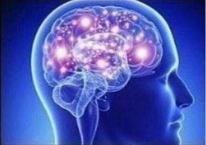
\includegraphics[scale = .6]{brain2}
 \end{center}


 \item Write somewhat useful programs by allowing the user and system to interact with the program through BIOS interrupts

 \begin{center}
  
\includegraphics[scale = .6]{brain3}
 \end{center}

\end{itemize}

 \end{frame}

 \begin{frame}{Goal: A $\lambda$-compiler}
  \begin{itemize}
    \item Write a $\lambda$-operating system
    \item Take over the world and assert $\lambda$-dominance
  \end{itemize}
 \begin{center}
  
\includegraphics[scale = 1.4]{brain4}
 \end{center}
 \end{frame}

  \begin{frame}{Lambda Calculus: A recapium}
 A $\lambda$-term is a term generated from:
 \[e ::= \lambda x . e \mid e \; e \mid x\]
But we don't like $x$: De Bruijn!
\[e ::= \lambda. e \mid e \; e \mid \L n\]

\begin{block}{Examples}

\end{block}

\begin{columns}
\begin{column}{0.5\textwidth}
 \[\lambda x . \lambda y . x + y\]
 \[ \lambda s. \lambda z. s\;s\;s\;s\;z \]
 \[\lambda f. (\lambda x . f(x\;x))(\lambda x . f(x\;x))\]
\end{column}

\begin{column}{0.5\textwidth}
 \[\lambda .\lambda . \L 1 + \L 0\]
 \[ \lambda. \lambda. \L 1 \; \L 1 \; \L 1 \; \L 1 \; \L 0 \]
  \[\lambda. (\lambda . \L1(\L0\;\L0))(\lambda . \L1(\L0\;\L0))\]
\end{column}
\end{columns}
 \end{frame}

 \begin{frame}{x86 Assembly: A recapium}
  \begin{itemize}
   \item Assembly language instruction map almost directly to CPU instructions
   \item You have freedom... and responsibilities.
  \end{itemize}
 \begin{center}
  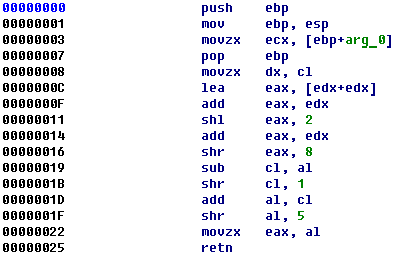
\includegraphics[scale = .6]{asm}
 \end{center}
 \end{frame}


 \begin{frame}[fragile]{BIOS}
 \begin{framed}
  \begin{center}\huge
   \textbf{B}asic \textbf{I}nput \textbf{O}utput \textbf{S}ystem
  \end{center}
 \end{framed}

  \begin{itemize}
   \item Provides a bunch of utilities to print to screen, read/write to disk, interact with hardware and peripherals, set timers, get info on memory....
   \item These different utilities can be invoked using \textbf{interrupts}.
  \end{itemize}
\begin{framed}
   \begin{verbatim}
  mov ah, 0x0E      ; Sets printing mode
  mov al, 'X'       ; Sets parameter of routine
  int 0x10          ; Calls interrupt, prints X
   \end{verbatim}
\end{framed}


 \end{frame}


 \begin{frame}{The language}
 The $\lambda$-calculus is cool and all, but we need to extend it a bit, with:
 \begin{itemize}
  \item Natural numbers
  \[\lambda. (5 * \L0)\]
  \item Conditionals
  \[ \lambda.(\texttt{if } \L0 = 7 \texttt{ then } 2 \texttt{ else } 9)\]
  \item Tuples
  \[(1, 5, 2, 4, 8)\]
  \item Effects!
  \[\texttt{INT}(1, 5, 2, 4, \lambda. 0)\]
 \end{itemize}

 \end{frame}

 \begin{frame}{Writing a (bad) compiler}
\begin{framed}
{\huge \[\lambda \longrightarrow \texttt{out.asm}\]}
\end{framed}


  Structure of the executable:
  \begin{itemize}
   \item The first 512 bytes of the executable consist of the \textbf{boot sector} of our bootable disk.
   \item In this sector we read the disk, load the rest of the executable and jump to it.
   \item Once jumped to the \emph{second stage bootloader}, the execution of our program starts.
  \end{itemize}

 \end{frame}

 \begin{frame}{The stacks}
  Each generated program acts on three stacks:
  \begin{itemize}
   \item The built-in stack \hfill(used for calling functions)
   \item The operand stack \hfill(used for performing operations)
   \item The AR stack \hfill(used for holding params and return addr)
  \end{itemize}\medskip

  For the latter two stacks, we define the following pointers:

  \begin{center}
   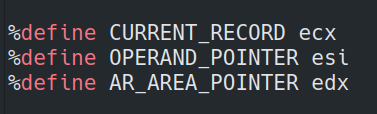
\includegraphics[scale = .7]{pointers}
  \end{center}

 \end{frame}

 \begin{frame}{Pushin' n' poppin'}
We define NASM macros for generating push and pop code for the various stacks, e.g.:
 \begin{center}
   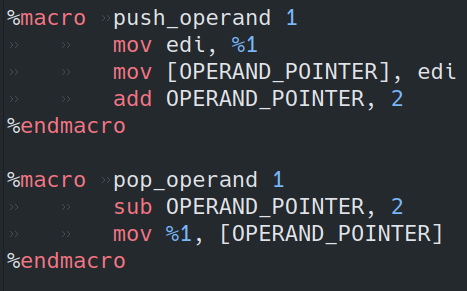
\includegraphics[scale = .7]{pushpop}
  \end{center}
 \end{frame}

\begin{frame}{Compiling arithmetic operations}

\end{frame}


\end{document}
